\chapter{Results and Discussion}\label{Results}

After completing an implementation of the design in Chapter~\ref{Implementation}, an evaluation of its effectiveness is conducted based on the goals of the project. In this chapter, a method for data collection using the implementation is presented, the results of the data collection are analysed, and a discussion on the overall strengths and weaknesses of the design and implementation is given. In particularly, the solutions ability to fairly balance load between co-operating TLS servers, minimising impact to overall network performance and demonstrating protection of user privacy are considered.





\section{Data Collection}

Wireshark is a tool for capturing and analysing network traffic. In this project, it is used to record all traffic passing through the bridge network. This includes traffic entering and leaving the virtual environment as well as traffic passed through the WireGuard VPN. Fig.\ref{wireshark_screenshot_figure} displays a few capabilities of the software, including presentation of all captured packets, filtering packets by content and recognition of the ECH extension in a ClientHello message.

\begin{figure}[ht]
\centerline{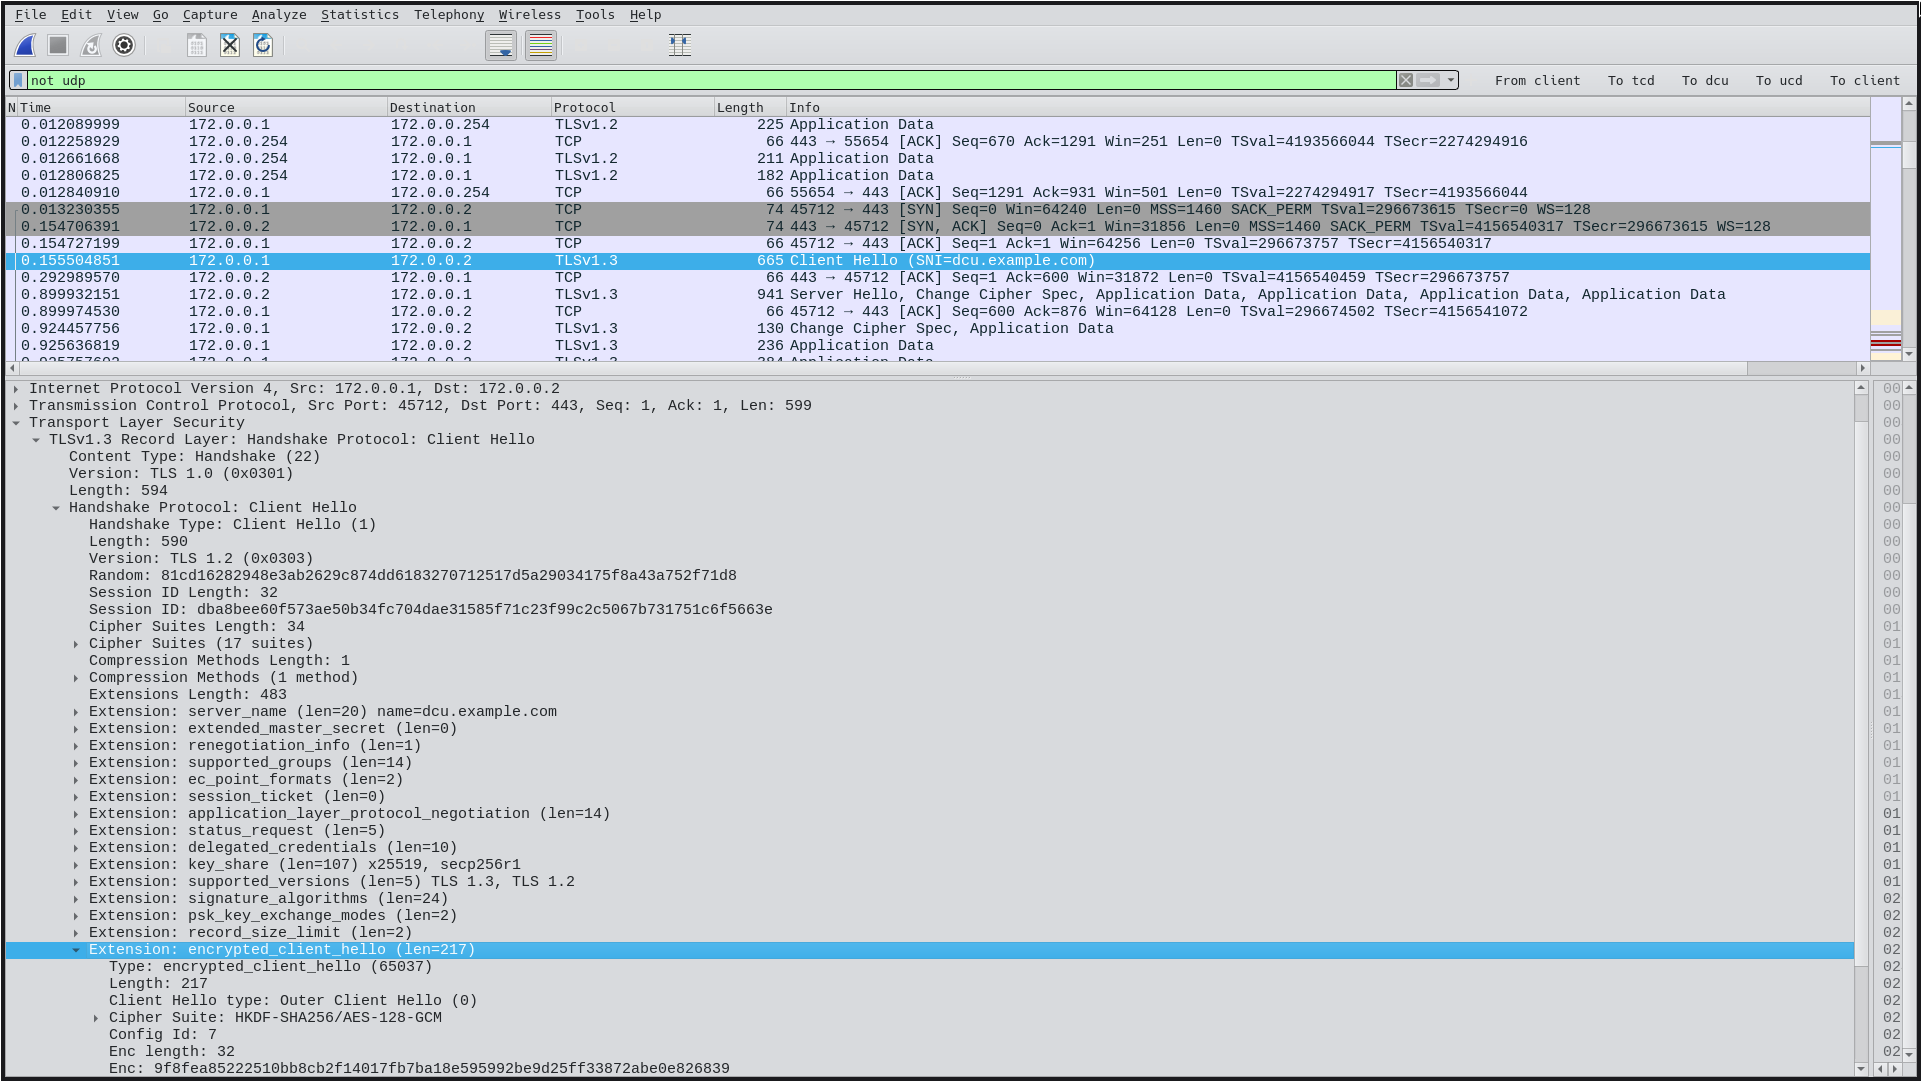
\includegraphics[width=120mm]{images/wireshark.png}}
\caption[Screenshot of Wireshark after capturing a Client Hello message using ECH]{Screenshot of Wireshark after capturing a Client Hello message using ECH.}
\label{wireshark_screenshot_figure}
\end{figure}









\section{Evaluation}

In this section we use the data captured using WireShark to consider and criticise various parts of the system in operation.
The collected data PCAP files have been included in the additional data ZIP archive submitted alongside this report.
% This data is collected in , which will be indicated when appropriate.


\subsection{Load Distribution}

The design appears to have achieved its objective of delivering load fairly across members of the co-operative network. Fig.~\ref{load_graph_figure} shows a very stable load persisting for 25 minutes. In this scenario, 60\% of traffic was destined to the blue origin server, while the other two servers shared the remaining 40\%. Due to the functionality of the dynamic DNS service, this difference in popularity is not noticeable. While this implementation is extremely simple and does not attempt to make intelligent decisions based on live traffic flow recordings, it does provide preliminary evidence that a dynamic DNS service can be used as a distribution mechanism for the distributed deployment of ECH.

\begin{figure}[ht]
\centerline{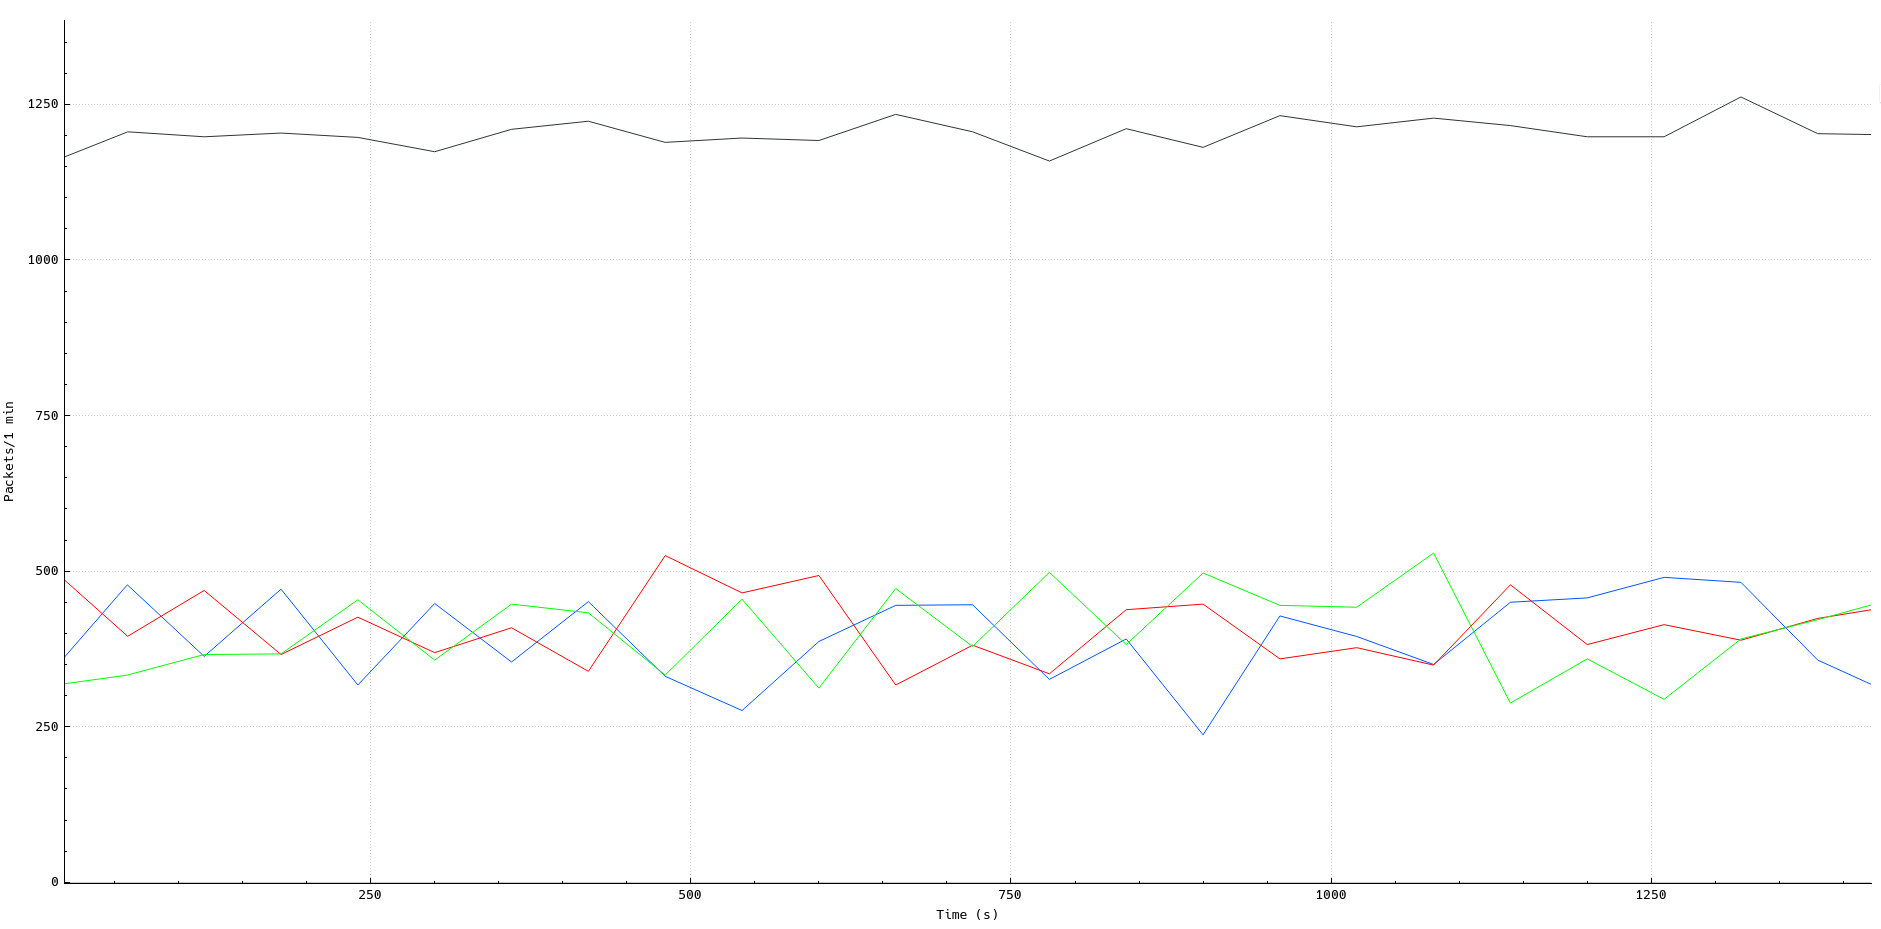
\includegraphics[width=120mm]{images/load.png}}
\caption[Load distribution graph]{Load experienced by three co-operative TLS servers from clients over a period of 25 minutes. The black line represents the total load bared across the whole network.}
\label{load_graph_figure}
\end{figure}




\subsection{Performance}

Data was also collected regarding the performance of scenarios where clients ignore ECH support and go straight to the origin and conventional ECH using a single centralised provider. We can see in Fig.~\ref{performance_graph_figure} and Table ~\ref{performance_table} that the distributed deployment model faired just as well as the centralised deployment model. When compared against no ECH usage, clearly the addition of traffic padding and a intermediate node significantly impacts performance. However, this is to be expected as ECH necessitates a intermediate node when using Split Mode. Overall, this result is a great success for the deployment model.

\begin{figure}[ht]
\centerline{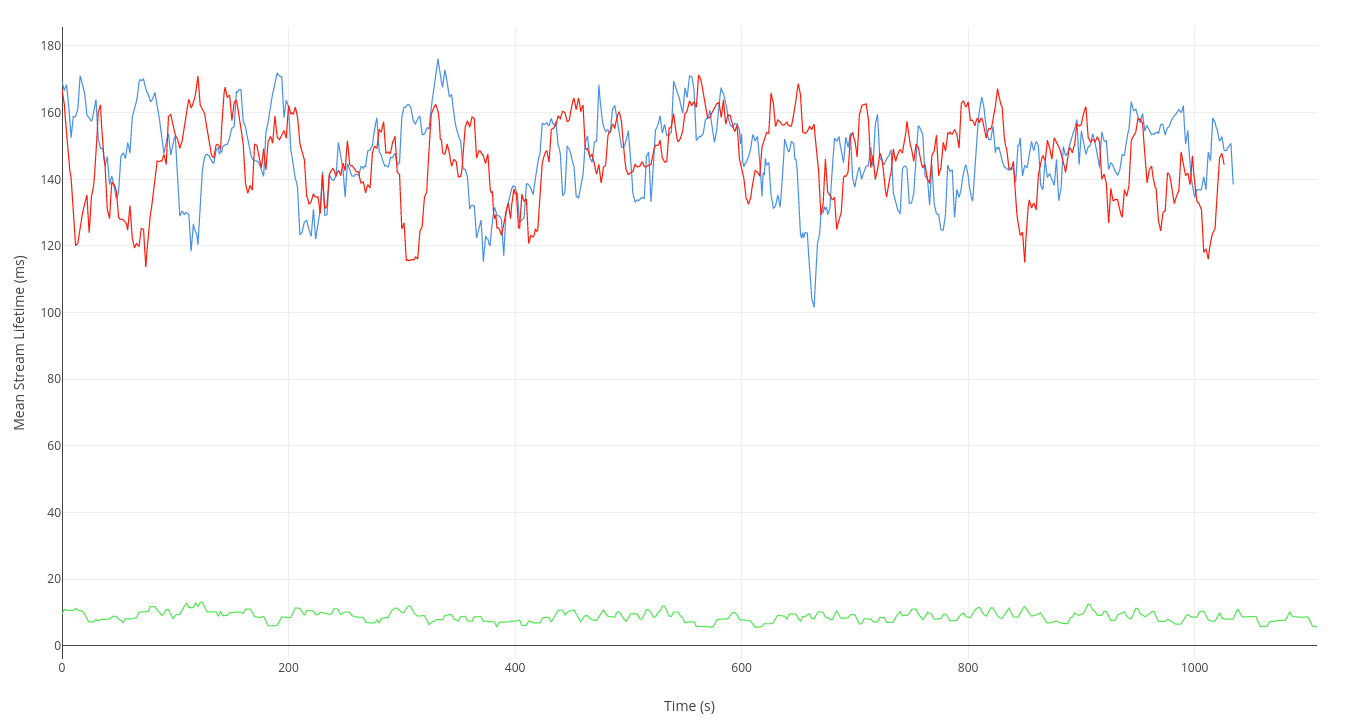
\includegraphics[width=120mm]{images/performance.png}}
\caption[Performance comparison graph]{Total time taken to fetch a resource within different scenarios. Blue is using distributed ECH, red is using centralised ECH and green is disregarding ECH and going straight to the origin server.}
\label{performance_graph_figure}
\end{figure}


\begin{table}[!h]
\begin{center}
\begin{tabular}{|r|r|r|r|}
\hline
\bf Statistic & \bf Distributed ECH & \bf Centralised ECH  & \bf Without ECH \\
\hline
\it \# streams (packets) & 1054 (11092) & 1046 (11017) & 1128 (11864) \\
\hline
\it Minimum lifetime & 13.7682 ms & 40.6940 ms & 4.6399 ms \\
\hline
\it Maximum lifetime & 255.2350 ms & 254.2059 ms & 23.5630 ms \\
\hline
\it Mean lifetime & 147.4227 ms & 146.3109 ms & 8.8034 ms \\
\hline
\it Standard deviation & 40.6287 ms & 38.6486 ms & 5.1609s ms \\
\hline
\end{tabular}
\end{center}
\caption[Table of performance characteristics]{Table of performance characteristics}
\label{performance_table}
\end{table}

\subsection{Security}

As mentioned previously, the traffic obfuscation aspect of this project was not able to finalise an implementation in time.
However, we can still see its attempt at preventing an obvious correlation between the red and blue server transmissions in Fig.~\ref{security_graph_figure}. Unfortunately, the current implementation of traffic obfuscation does not mesh well with WireGuard, as a key exchange occurs before tcpdump has time to notice channel activity. Thus, there is always a clear relationship between the two communicators. Another method not implemented but researched is the constant injection of noise that adapts in volume with activity on the channel.


\begin{figure}[ht]
\centerline{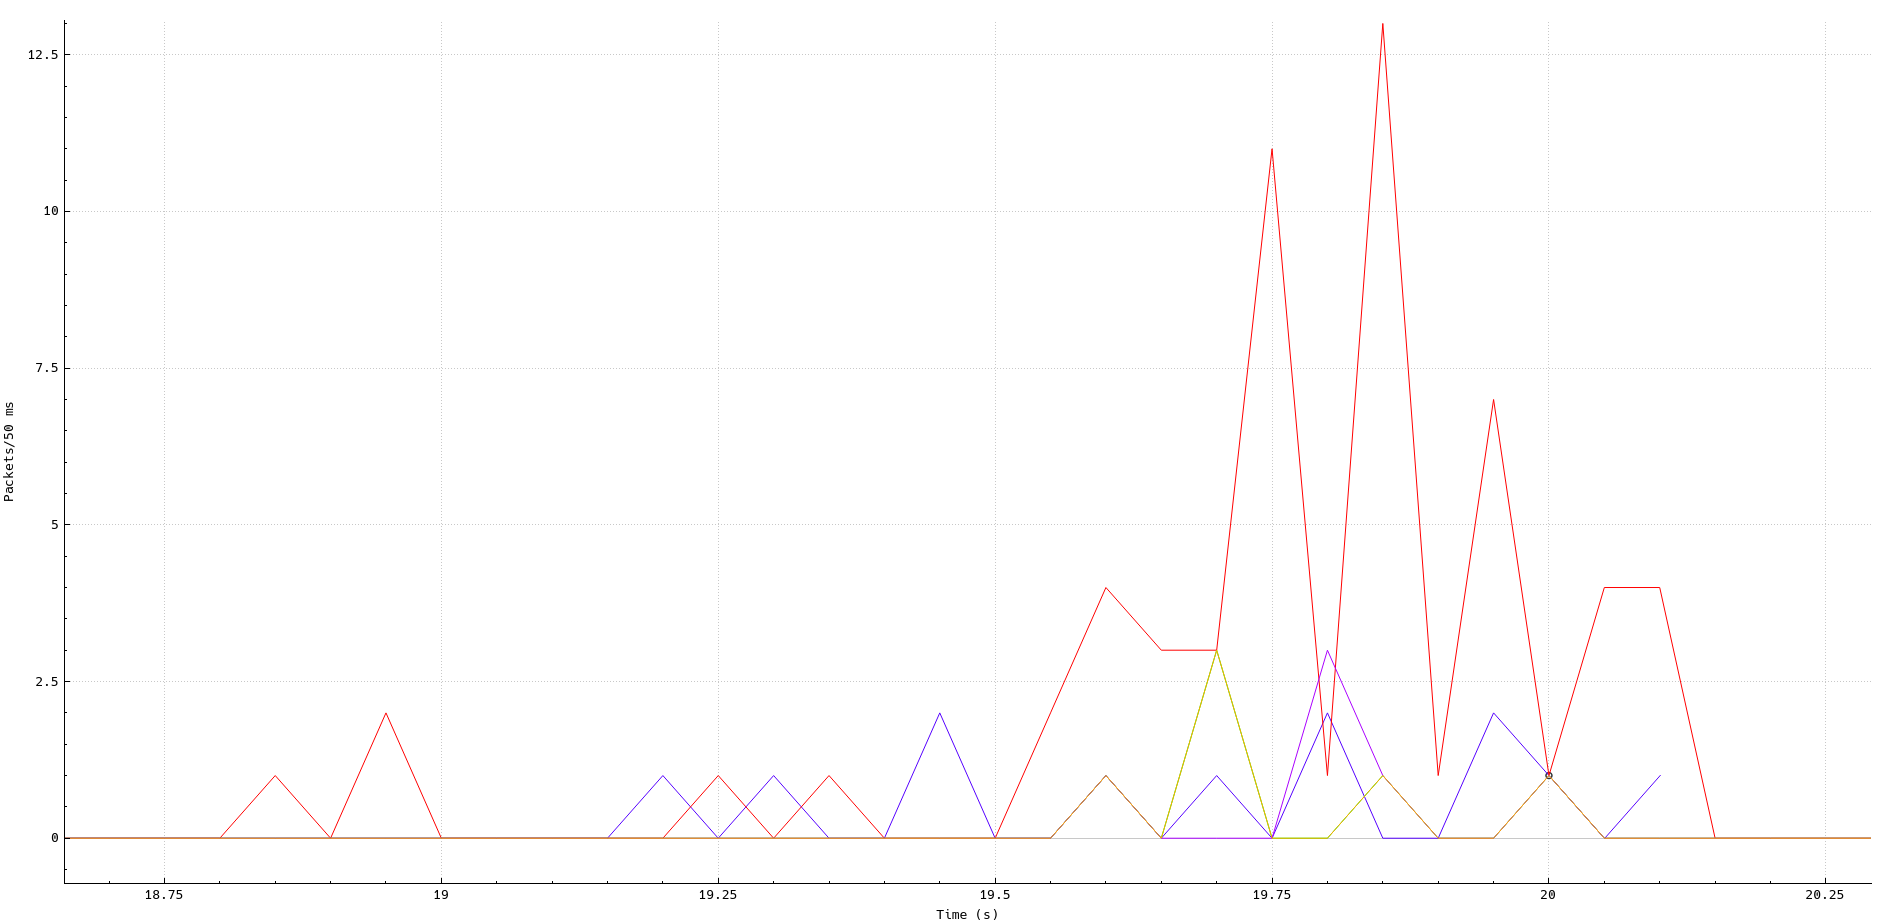
\includegraphics[width=120mm]{images/security.png}}
\caption[Impact of traffic obfuscation]{Impact of traffic obfuscation}
\label{security_graph_figure}
\end{figure}








\section{Summary}

The results from this study appear to be promising. The mechanism used for load balancing has archived its objective and distributed deployment does not appear to be negatively effecting network performance. While WireGuard has successfully concealed the ClientHelloInner when being forwarded, it still remains to be seen if the protocol can be operated in such a scenario without being compromised through traffic correlation.
